Energieeffizienzsteigerung ohne Sensorsysteme ist undenkbar. Dieses Kapitel stellt mehrere Arbeiten vor die sich auf die zwei Hauptformen der Datenerfassungssysteme für Landwirtschaftsplanungssysteme:

\begin{itemize}
	\item Sensornetzwerke
	\item GIS-Systeme
\end{itemize}

Dafür werden Arbeiten vorgestellt die sich mit der Effizienz der Sensornetzwerkysteme sowie mit den effizientesten Netzwerktopologien beschäftigen.

Anschließend werden Grundbegriffe der Geoinformatik erläutert und Arbeiten aus diesem Fachgebiet die mit Energieeffizienz in der Landwirtschaft in Beziehung stehen vorgestellt. 

\section{Sensornetzwerke als Datenquellen}
Sensortechnologie wurden im Laufe des AGREE-Projekts zum wichtigsten Forschungsgebiet in der zu zukünftigen Zusammenarbeit gewählt.\cite{misc:Mikkola2013} Sensornetzwerke sind Netzwerke aus Knoten die folgende bestimmte Funktionen verfügen bzw. folgende Bestandteile haben:
\begin{itemize}
	\item Sensoren um verschiedene Umweltparameter messen zu können. (z.B. Luftdruck, Luftfeuchtigkeit, Zusammensetzung der Gase in Umgebungsluft, Helligkeit, etc.)
	\item Rechenmodule um bestimmte Kalkulationen durchzuführen um z.B. Sensorenwerte auszuwerten.
	\item Kommunikationsmodule um entweder Messungen oder (Teil-)Ergebnisse von Kalkulationen zu übermitteln. (z.B. ZigBee, Wireless Lan, etc.)
\end{itemize}
Wenn diese Funktionen um ein Modul zur Fortbewegung des Knotens erweitert wird, handelt es sich um einen mobilen Sensornetzwerkknoten.\cite{jour:Howard2002}

Die Sensormodule können je nach Einsatzzweck sowohl in kleinen, gut zu kontrollierenden Bereichen wie z.B. Glashäusern eingesetzt werden, in großflächigen Feldern oder in Ställen in der Viehhaltung. Dies ist eine notwendige Basis für sg. \textit{Context Aware Computing}-Anlagen die bestimmte Umweltparameter wie z.B. Licht, Nahrung oder Bewässerung steuern können. 

Energieeffizienz spielt für Sensorknoten im Falle von Einsätzen auf großflächigen Feldern eine besondere Rolle, da hier der Einsatz von Batterien bzw. Akkumulatoren eine Notwendigkeit ist und die Wartung bzw. das Austauschen oder Aufladen aufwendig. 

In \cite{conf:Zia2013} werden drei \textit{Media Access Control}-Protokolle, kurz MAC, vorgestellt (ECR-MAC, EECR-MAC, EQR-MAC) die für den Einsatz für Adhoc-Sensornetzwerke konzipiert wurden. In \cite{jour:Jelicic2013} werden Optimierung sowohl was das Netzwerkprotokoll bis hin zum Physical Layer betrifft vorgestellt aber auch was den Energiehaushalt des Knoten betrifft. Dabei wird eine Lebenszeit von mehreren Jahren für einen Knoten erreicht.

In \cite{jour:Nandurkar2014} wird eine Beispiel-Implementierung eines Sensor-Netzwerks zur optimalen Wasserversorgung vorgestellt. Die Autoren kamen zu dem Ergebnis dass sowohl der Ernteertrag gesteigert werden konnte sowie Wasser-, Energie- und Arbeitsaufwand gemindert werden konnten.

Bhargava untersucht in \cite{jour:Bhargava2014} wie das Netzwerk am effizientesten aufgebaut werden kann und geht auf die Auswertung der gemessenen Daten ein. Er unterscheidet grob zwischen zwei Architekturen:
\begin{itemize}
	\item Die sg. \textit{Two-Tier-Architecture}
	\item Einem \textit{Peer to Peer Netzwerk} kurz P2P
\end{itemize}

Die Two-Tier-Architektur, siehe Abbildung \ref{fig:two_tier_architecture}, ist die Aufteilung von Sensor-Netzwerk und Intelligenz. Dabei sind die Tiers durch das Internet verbunden was die Auswertung in Cloud-Services erlauben würde. Neben dem Vorteil die Auswertung aus dem Betrieb auslagern zu können, erlaubt diese Aufteilung die Knoten langlebiger betreiben zu können. Der Autor stellt fest, dass auf den Sensorknoten eine jede Berechnung auf Kosten der verfügbaren Akkuleistung geht.\cite{jour:Bhargava2014}

\begin{figure}[h]
 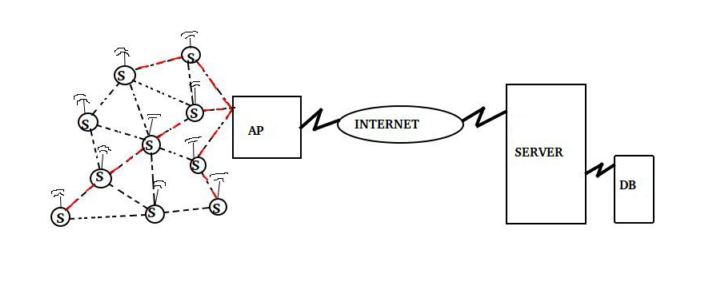
\includegraphics[scale=0.65,natwidth=\textwidth]{figures/sensors/two_tier_architecture.png}
 \centering
 \label{fig:two_tier_architecture}
 \caption{Vorgeschlagene Two-Tier-Architektur \cite{jour:Bhargava2014}}
\end{figure}

Im Gegensatz dazu, werden die gemessenen Daten in der P2P-Architektur (dargestellt in Abbildung \ref{fig:p2p_architecture_img}) im Netzwerk ausgewertet. Dies hat im Vergleich zur Two-Tier-Architektur Nachteile:
\begin{itemize}
	\item Die Lebensdauer der verwendete Energiequelle leidet darunter und ist früher erschöpft.
	\item Es können durch die begrenzte Leistungsfähigkeit der verfügbaren Chips auf den Sensorknoten nur triviale Auswertungen durchgeführt werden.
	\item Je nach Einsatzgebiet (z.B. in gebirgigen Landschaften), kann die Verfügbarkeit der Daten nicht garantiert werden. Dies könnte bei einem Alarm dazu führen, dass dieser zu spät gemeldet werden kann.
\end{itemize}

\begin{figure}[h]
 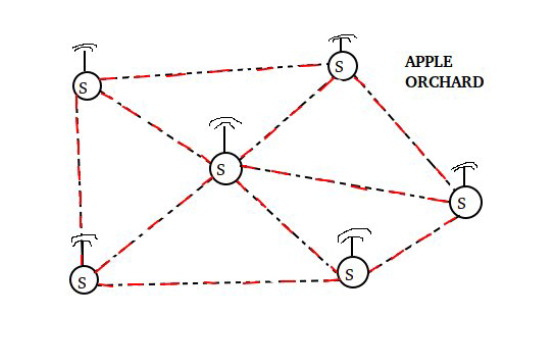
\includegraphics[scale=0.75,natwidth=\textwidth]{figures/sensors/p2p_architecture.png}
 \centering
 \label{fig:p2p_architecture_img}
 \caption{P2P-Struktur des Sensornetzwerks \cite{jour:Bhargava2014}}
\end{figure}

Aus diesen Gründen spricht Bhargava die Empfehlung aus, die Auswertung auf einen Server welcher über das Internet erreichbar ist auszulagern.

In \cite{jour:Srbinovska2014} wird ein Sensornetzwerk für ein Paradeiserglashaus entworfen. Die verwendeten Sensoren maßen die Temperatur, Erdfeuchtigkeit und pH-Wert der Erde. Im Unterschied zu Bhargava wurde ein Gossip-Protokoll zur Kommunikation innerhalb des Sensornetzwerks verwendet.

Gossip-Protokolle sind definiert durch eine Netzwerktopologie ohne Superknoten. Die einzelnen Knoten besitzen einen lokalen Zustand der im Netzwerk mittels Broadcasts in definierten Abständen mitgeteilt wird. Dies hat zur Folge, dass einzelne Knoten ohne Aufwand hinzugefügt oder entfernt werden können. Dieses Vorgehen hat Vorteile da keine Superknoten benötigt werden die das Routing übernehmen, ist energieaufwendig. Die Energieaufnahme versucht Pazurkiewicz in \cite{jour:Pazurkiewicz2014} mit seinem NarrowCast-Protokol zu mindern.

Srbinovska und seine Kollegen haben sich für ein Gossip-Protokoll in ihrem Testaufbau entschieden, da für das System ein Temperaturdurchschnittswert interessant ist. Durch die Broadcasts der jeweilig lokal gemessenen Temperaturen wurden lokal auf den Knoten die Durchschnittswerte errechnet und gespeichert. Im Experiment wurde fest gestellt, dass die Durchschnittswerte der einzelnen Knoten annähernd dem tatsächlichen Wert entsprach. Dies dauerte zwischen 15 und 20 Broadcasts.\cite{jour:Srbinovska2014}

Die Autoren kamen abschließend zu dem Ergebnis, dass bei der Planung auf mehrere Aspekte geachtet werden muss.\cite{jour:Srbinovska2014}
\begin{itemize}
	\item Auswahl des effizientesten Frequenzbereichs für die Funkverbindung. Die Frequenz der WiFi-Transmitter ist entscheidend für die Energieeffizienz der Sensor-Knoten.
	\item Die Preise der verfügbaren Hardware-Module ist zu hoch.
	\item Vor dem Ausrollen solcher Sensornetzwerke in großen Anlagen, müssen weitere Pilotprojekte durchgeführt werden um den Erfolg nicht zu gefährden.
\end{itemize}

Neben den erwähnten Sensoren wird in \cite{jour:Romeo2013} ein System vorgestellt, dass in der Lage ist auf Basis von Bilddaten Entscheidungen zu treffen. Die Auswertung setzt qualitativ hochwerte Bilder als Basis voraus. Die Bewertung und Planung der Aktionen wird von einem Expertensystem durchgeführt.

\section{Satellitensysteme als Datenquellen}

Geoinformationssysteme, sind Informationssysteme die Lageinformationen verarbeiten, aufbereiten und bereitstellen. In der Literatur wird zwischen vier verschiedenen Definitionen unterschieden:\cite{book:Carosio2006}

\begin{itemize}
	\item \textit{Raumbezogene Informationssysteme}, kurz RIS, sind laut \cite{book:Cariosio2006} geordnete Sammlungen von Informationen, in welchen Lagenangaben in einem einheitlichen Bezugssystem eine Verknüpfung zwischen den enthaltenen Daten und der Umwelt ermöglichen.
	\item \textit{Geographisches Informationssystem}, kurz GIS, ist ein Informationssystem das raumbezogene Daten über Atmosphäre, Erdoberfläche, Lithosphäre enthält. Zusätzlich ermöglicht ein GIS die systematische Erfassung, Aktualisierung, Verarbeitung und Umsetzung der Daten auf der Grundlage eines einheitlichen räumlichen Bezugssystems.
	\item \textit{Landinformationssysteme}, kurz LIS, sind Informationsysteme die bei Fragen in der Verwaltung, Wirtschaft oder Rechtsproblemen Auskünfte geben können. 
	\item \textit{Geoinformationssysteme}, kurz ebenfalls GIS, sind rechnergestützte Systeme die aus Hardware, Software, Daten und der Anwendung bestehen. Diese Systeme können genutzt werden raumbezogene Daten digital zu erfassen, modellieren, reorganisieren, analysieren und alphanumerisch und graphisch präsentieren können.
\end{itemize}

Die vorgestellten Publikationen verwenden die vierte Definition.

\subsection{Kenzahlen in GI-Systemen}
In \cite{jour:Vibhute2013} gibt Vibhute einen Überblick über verwendete Sensortechnologien und Kennzahlen die zur Auswertung heran gezogen werden können.  

\subsubsection{Landnutzungseffizenz}

Um zu ermitteln wie effizient der verfübgare Platz genutzt wird kann das Verhältnis von \textit{Land Use} zu \textit{Land Cover} heran gezogen werden. Land Cover ist die Kennzahl die beschreibt wie viel der Erdoberfläche von Material bedeckt ist. Dazu zählen Gras, Asphalt, Bäume, etc. Demgegenüber steht Land Use, was definiert wie viel der Erdoberfläche vom Menschen genutzt wird.

Die Rohdaten werden aus Satellitenbildern gewonnen. Die Elemente in den Bildern können mit verschiedenen Klassifierern zu Land Use bzw. Land Cover zugeordnet werden. Vibhute stellt Varianten in \cite{jour:Vibhute2013} vor. (z.B. Maximum-Likelyhood-Classifier, Supervised Classifier, etc.)

\subsubsection{Vegetationsindizes} 
Vegetationsindizes sind Kennzahlen die aus Messungen von elektromagnetischer Strahlung um das infrarote Spektrum herum gewonnen werde.\cite{jour:Jackson1991}

Vibhute stellt in \cite{jour:Vibhute2013} eine Tabelle \ref{table:gsi_indices} der verschiedenen Vegetationsindizes auf:

\begin{table}[h]
\label{table:gsi_indices}
\begin{tabular}{|p{5cm}|p{9cm}|}
\textbf{Vegetationsindex}                                  & \textbf{Formel} \\
RVI (Ratio Vegetation Index)                               & $RVI = \frac{NIR}{RED}$                 \\
NDVI (Normalized Difference Vegetation Index)              & $NDVI = \frac{NIR - RED}{NIR + RED}$                \\
NDWI (Soil Adjusted Vegetation Index)                      & $NDWI = \frac{NIR - SWIR}{NIR + SWIR}$                \\
SAVI (Soil Adjusted Vegetation Index)                      & $SAVI = \frac{(1 + L)(NIR - RED)}{NIR + RED + L}$                \\
TVI (Triangular Vegetation Index)                          & $TVI = \frac{120 (NIR - GREEN)}{2} - 200 (RED - GREEN)$                \\
TNDVI (Transformed Normalized Difference Vegetation Index) & $TNDVI = \sqrt[2]{\frac{NIR - RED}{NIR + RED} + \frac{1}{2}}$               
\end{tabular}
\end{table}

\subsection{Anwendungen von GIS-Technologien}

In \cite{jour:Huang2013} wird eine auf Satellitenbildern aufbauende Analyse des Reisanbaus vorgeschlagen. Dieses Vorgehen hat den Vorteil, dass zum einen die Gebiete nicht mit Sensorknoten bestückt werden müssen - was im Falle von Nassgebieten wie Reisfeldern weitere Probleme bereit hält - und dass die lokalen Messinstrumente nur über längere Zeitperioden verlässliche Daten liefern.

In \ref{fig:satellite_area} wird das Gebiet in dem die Datenmessung untersucht wurde dargestellt.

\begin{figure}[h]
 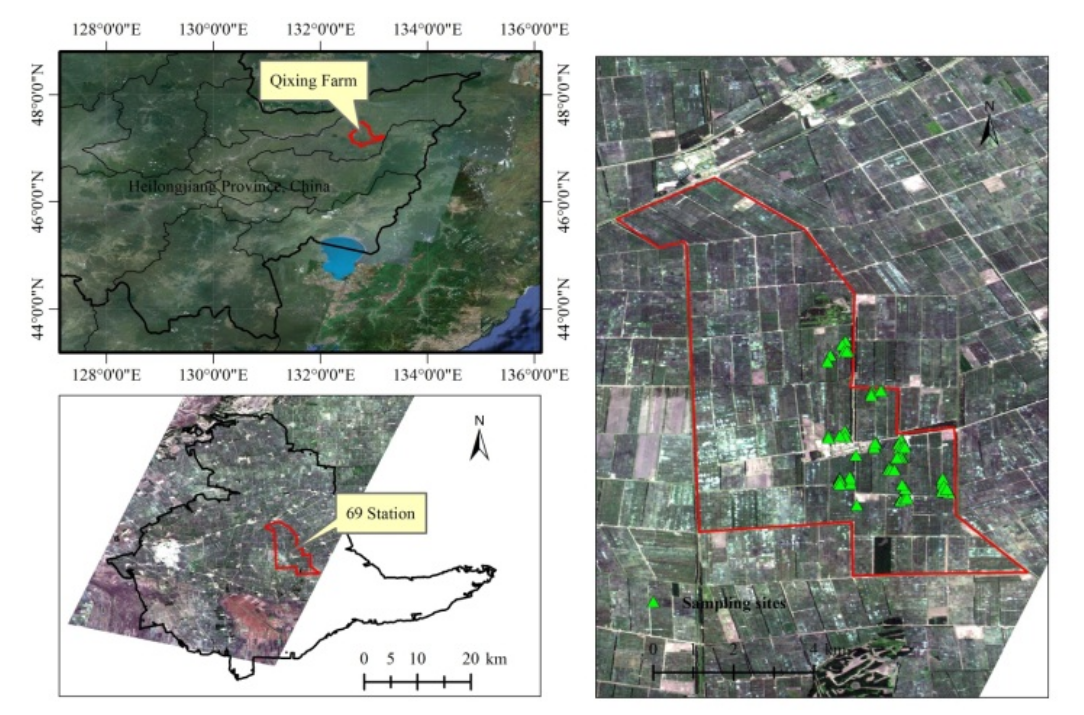
\includegraphics[scale=0.4,natwidth=\textwidth]{figures/sensors/satellite_area.png}
 \centering
 \label{fig:satellite_area}
 \caption{Aufnahme des Gebiets dessen Umweltwerte gemessen wurden. \cite{jour:Huang2013}}
\end{figure}

In \cite{jour:Omarova2013} gehen Omarova, Sennikov, Omarov und Kolbachaeva darauf ein wie großflächige Wetter und Landschaftsdaten genutzt werden können, den Ertrag von Zuckerrübenernten zu steigern. Dazu modellieren sie die Pflanzen um die nötigen Mengen an Wasser errechnen zu können und dies mit der vorhandenen Infrastruktur bestmöglich zu paaren.

Daten aus GIS-System ermöglichen einen großflächigeren Blick als lokale Sensoren. Mit \cite{book:Hou2013} wird gezeigt, dass dieser Ansatz dazu verwendet werden kann, die Produktionsunterschiede zwischen minderleistenden Gebieten und Gebieten mit hohem Ertrag zu ermitteln. Dies kann dazu genutzt werden die Prozesse in den minder leistenden Arealen zu erhöhen.

Der Stand der Forschung der Landschaftsanalyse und Modellierung wird in \cite{jour:Zhou2013} zusammen gefasst.

GIS-Daten über Grenzen (seien es Betriebsgrenzen, nationale Grenzen, etc.) hinweg nutzen zu können, muss eine Möglichkeit gefunden werden die Zusammenarbeit zu strukturieren. Nyerges, Roderick und Avraam stellen in \cite{jour:Nyerges2013} ein Survey vor dass die aktuelle Forschung umreißt. 

Neben den Satellitensystemen werden auch Flugzeuge zur Messung von Geodaten verwendet. In \cite{jour:Honkavaara2012} wird ein Drohnenexperiment vorgestellt, welches optische Sensoren verwendet um Informationen über die Anbaufläche zu sammeln.